\subsection{Messergebnisse und Auswertung}
\subsubsection{Bandlückenenergie von Silizium}
Das Spektrum der Absorption (gemessen mit der Silizium-Probe) und Transmission (gemessen mit dem Pyrodetektor) von Silizium 
in Abhängigkeit des Winkels $\alpha$ ist in \autoref{img:si:spectrum} dargestellt. Man erkennt das Maxima 0. Ordnung bei $\alpha = 0^\circ$. 
Durch diese Eichung des Winkels kann das verwendete Messprogramm die Winkel schon in die richtigen Energien 
(abhängig vom Winkel und der Gitterkonstante) umrechnen, welche später noch benötigt werden.
\begin{figure}[H]
\begin{center}
  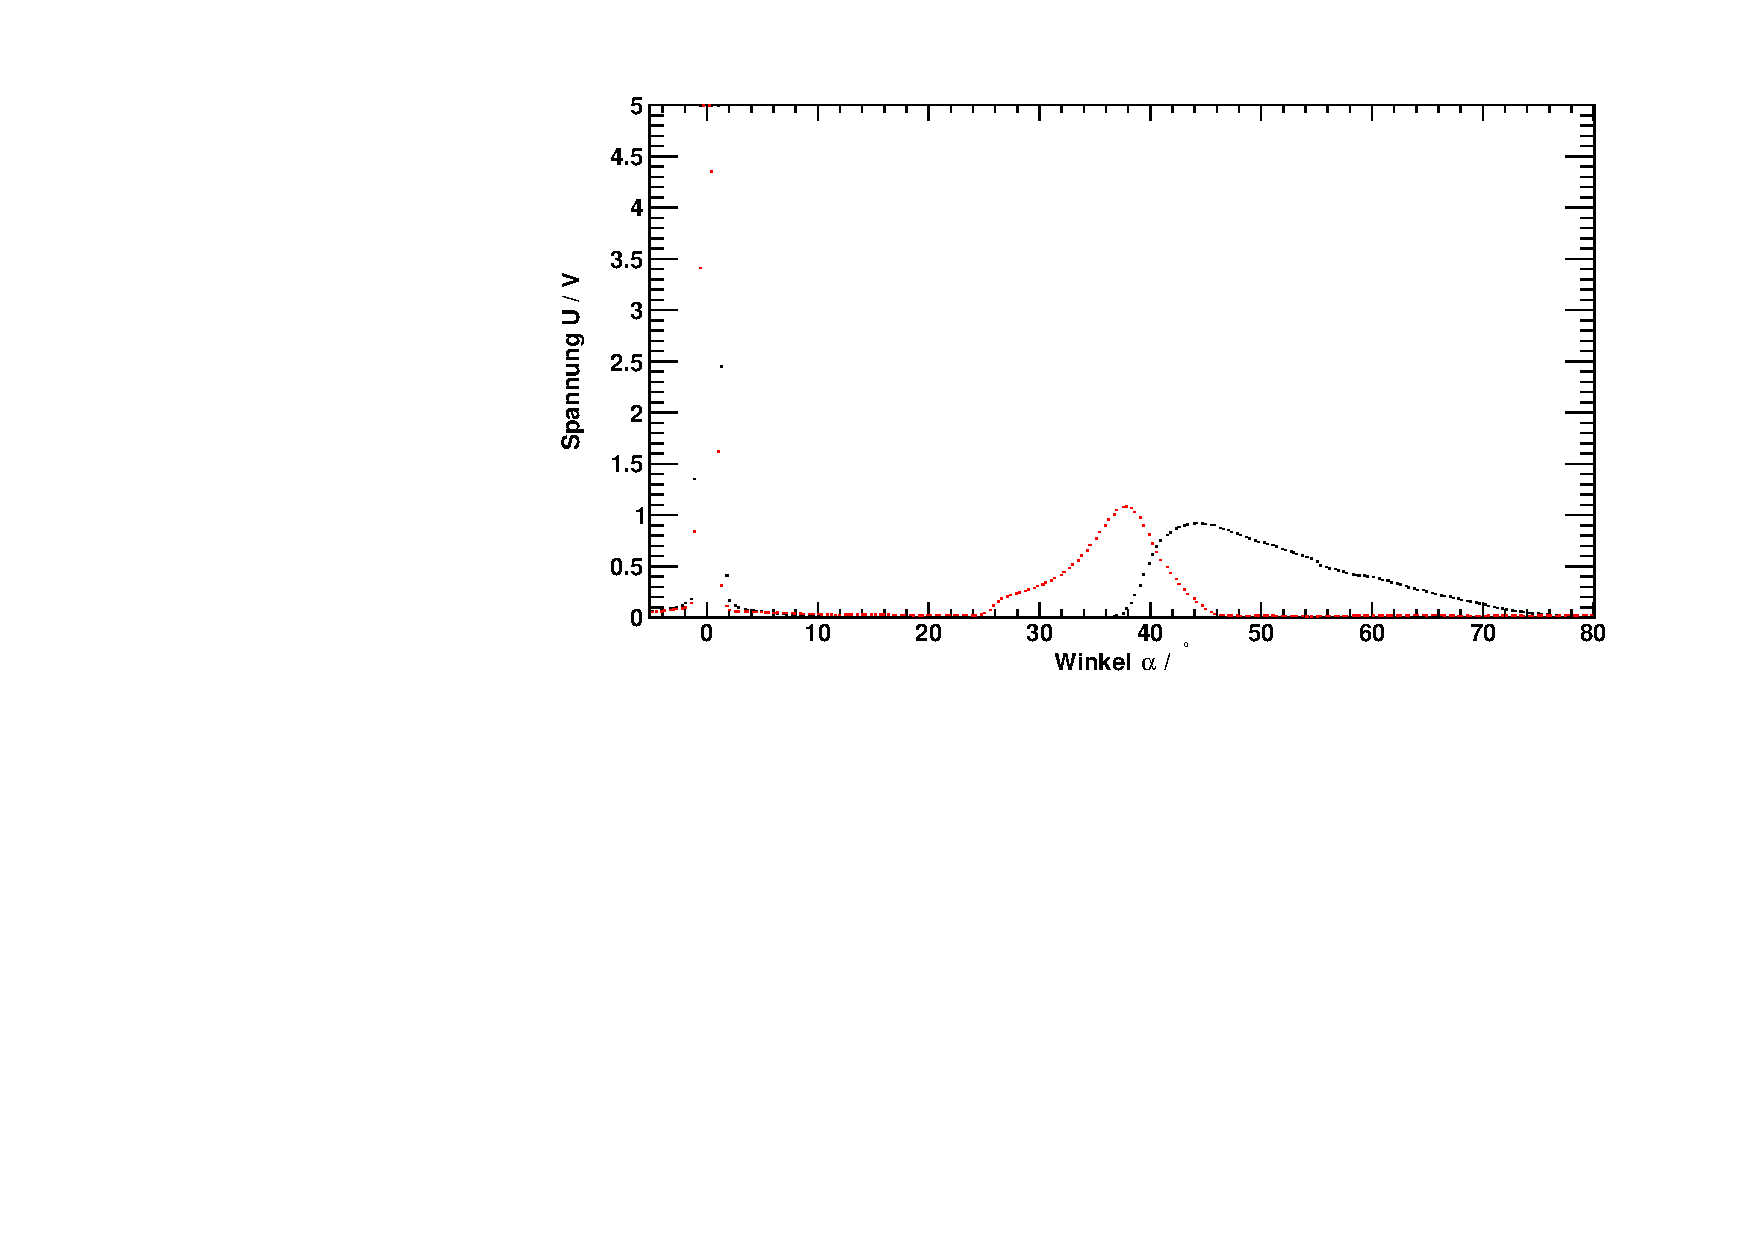
\includegraphics[width=\textwidth]{../img/part1/Si_Messung_spectrum.pdf}
  \caption{Absorptions- und Transmissionsspektrum von Silizium.}
  \label{img:si:spectrum}
\end{center}
\end{figure}

Für die Fehler der Messpunkte wurde die Spannung an den Sensoren über einen längeren Zeitraum ($t=100$\,s) bei den Winkeln der maximalen 
Transmission und Absorption gemessen. Aus dieser Messreihe wurde die Standardabweichung
\begin{equation}
  s_U = \sqrt{ \frac{1}{N - 1} \sum_{i=1}^N \left( \bar{U} - U_i \right)^2 }
\end{equation}
bestimmt und als absoluter Fehler der einzelnen Messpunkte gesetzt.
\begin{equation}
  s_{\text{Abs}} = 0.007\,\text{V}, \qquad s_{\text{Trans}} = 0.004\,\text{V}
\end{equation}

Um die Bandlückenenergie von Silizium zu bestimmen, muss von den beiden Messungen jeweils der Untergrund (\autoref{img:si:underground}) abgezogen 
werden. Des weiteren müssen die Messungen auf die Leistung der Lampe normiert werden, da diese nicht für alle Winkel gleich ist 
(\autoref{img:si:lampe}). Da die Winkel nur jede halbe Sekunde aufgenommen werden, sind die genauen Werte der Winkel nicht reproduzierbar. 
Deshalb wurde für jeden Messpunkt eine lineare Interpolation des Untergrunds und des Spektrums der Lampe zwischen den benachbarten Punkten 
durchgeführt.
\begin{equation}
  I_{\text{Pyro}} = \frac{U_{\text{Pyro}} - U_{\text{Untergrund,Pyro}}}{U_{\text{Lampe}}}, \qquad I_{\text{Probe}} = \frac{U_{\text{Probe}} - U_{\text{Untergrund,Probe}}}{U_{\text{Lampe}}}
\end{equation}
Die Fehler berechnen sich mit der Gauß'schen Fehlerfortpflanzung.

\begin{figure}[H]
\begin{center}
  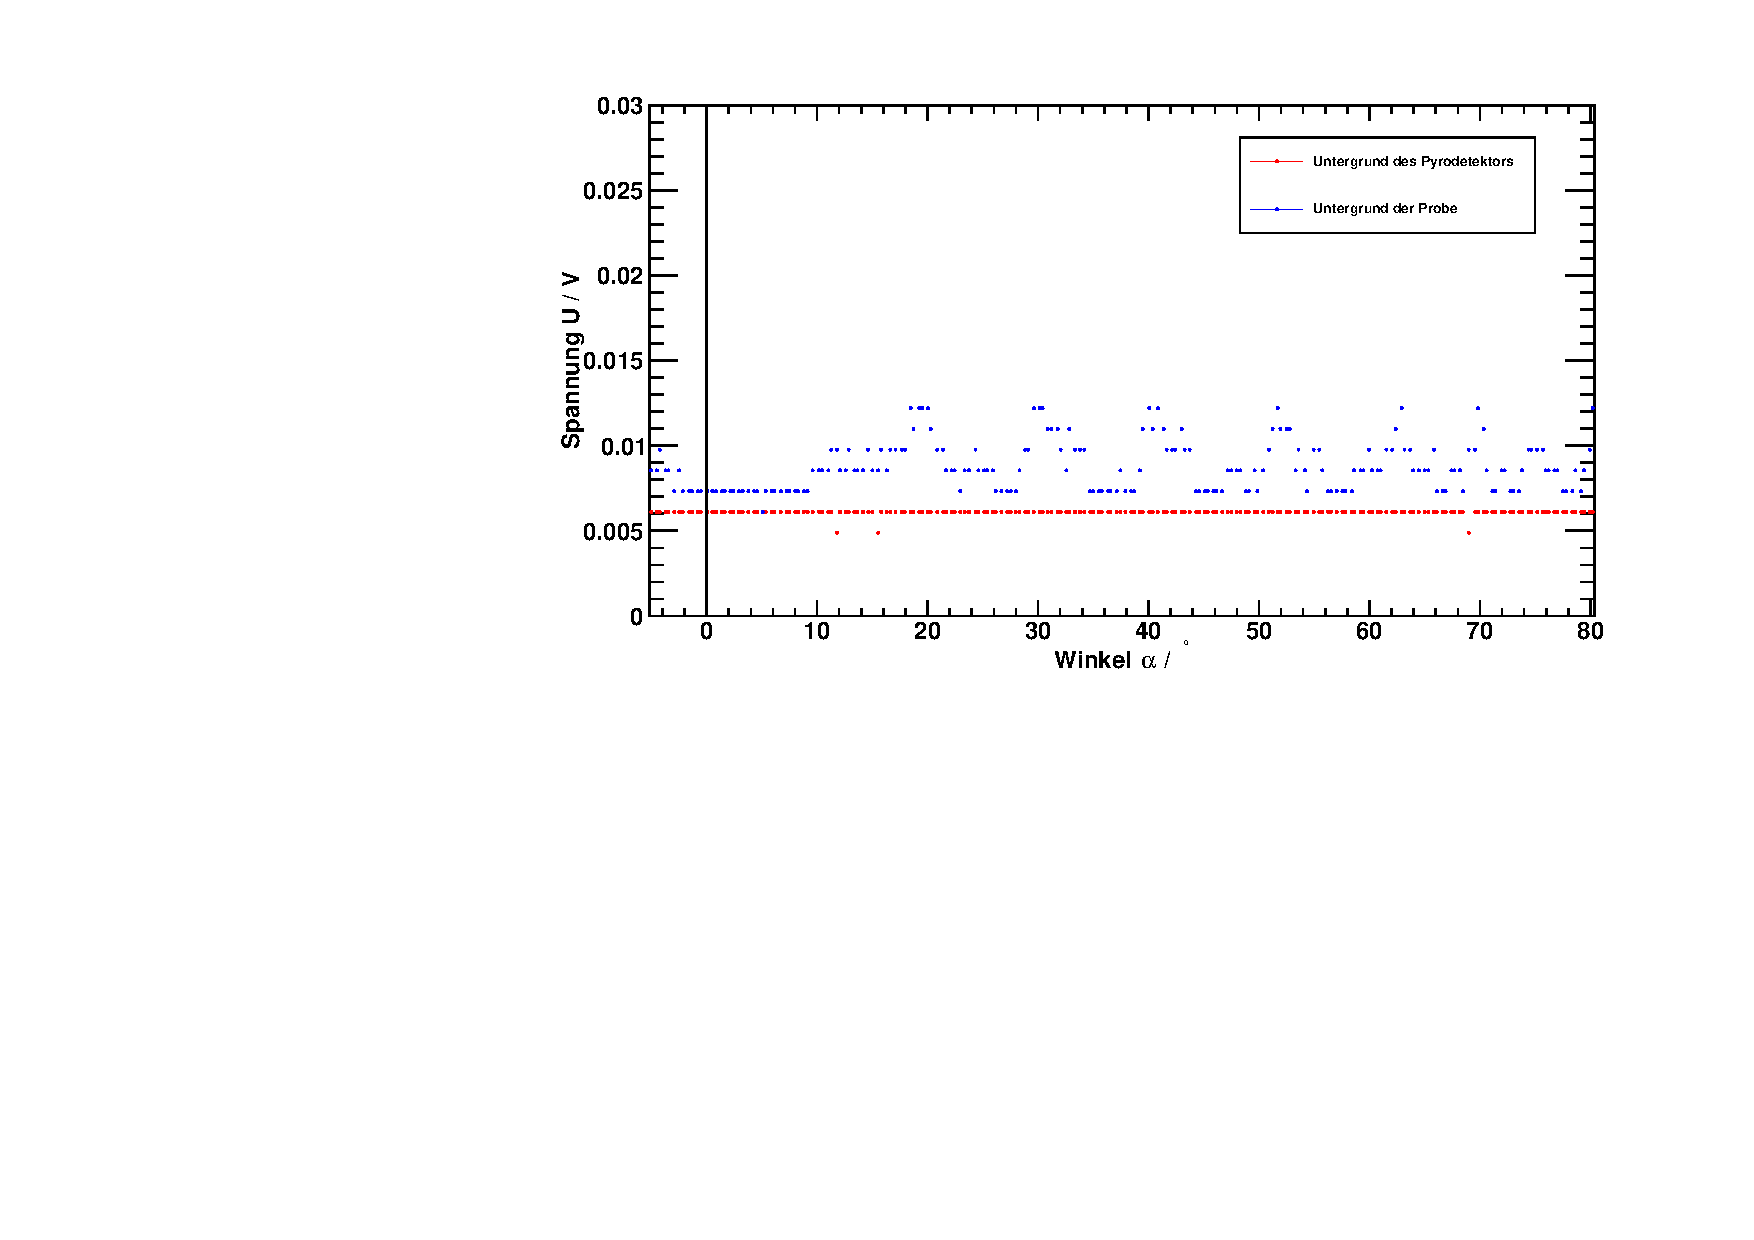
\includegraphics[width=\textwidth]{../img/part1/Si_Untergrund_spectrum.pdf}
  \caption{Untergrund von Pyrodetektor und Siliziumprobe, gemessen mit abgedeckter Lampe.}
  \label{img:si:underground}
\end{center}
\end{figure}

\begin{figure}[H]
\begin{center}
  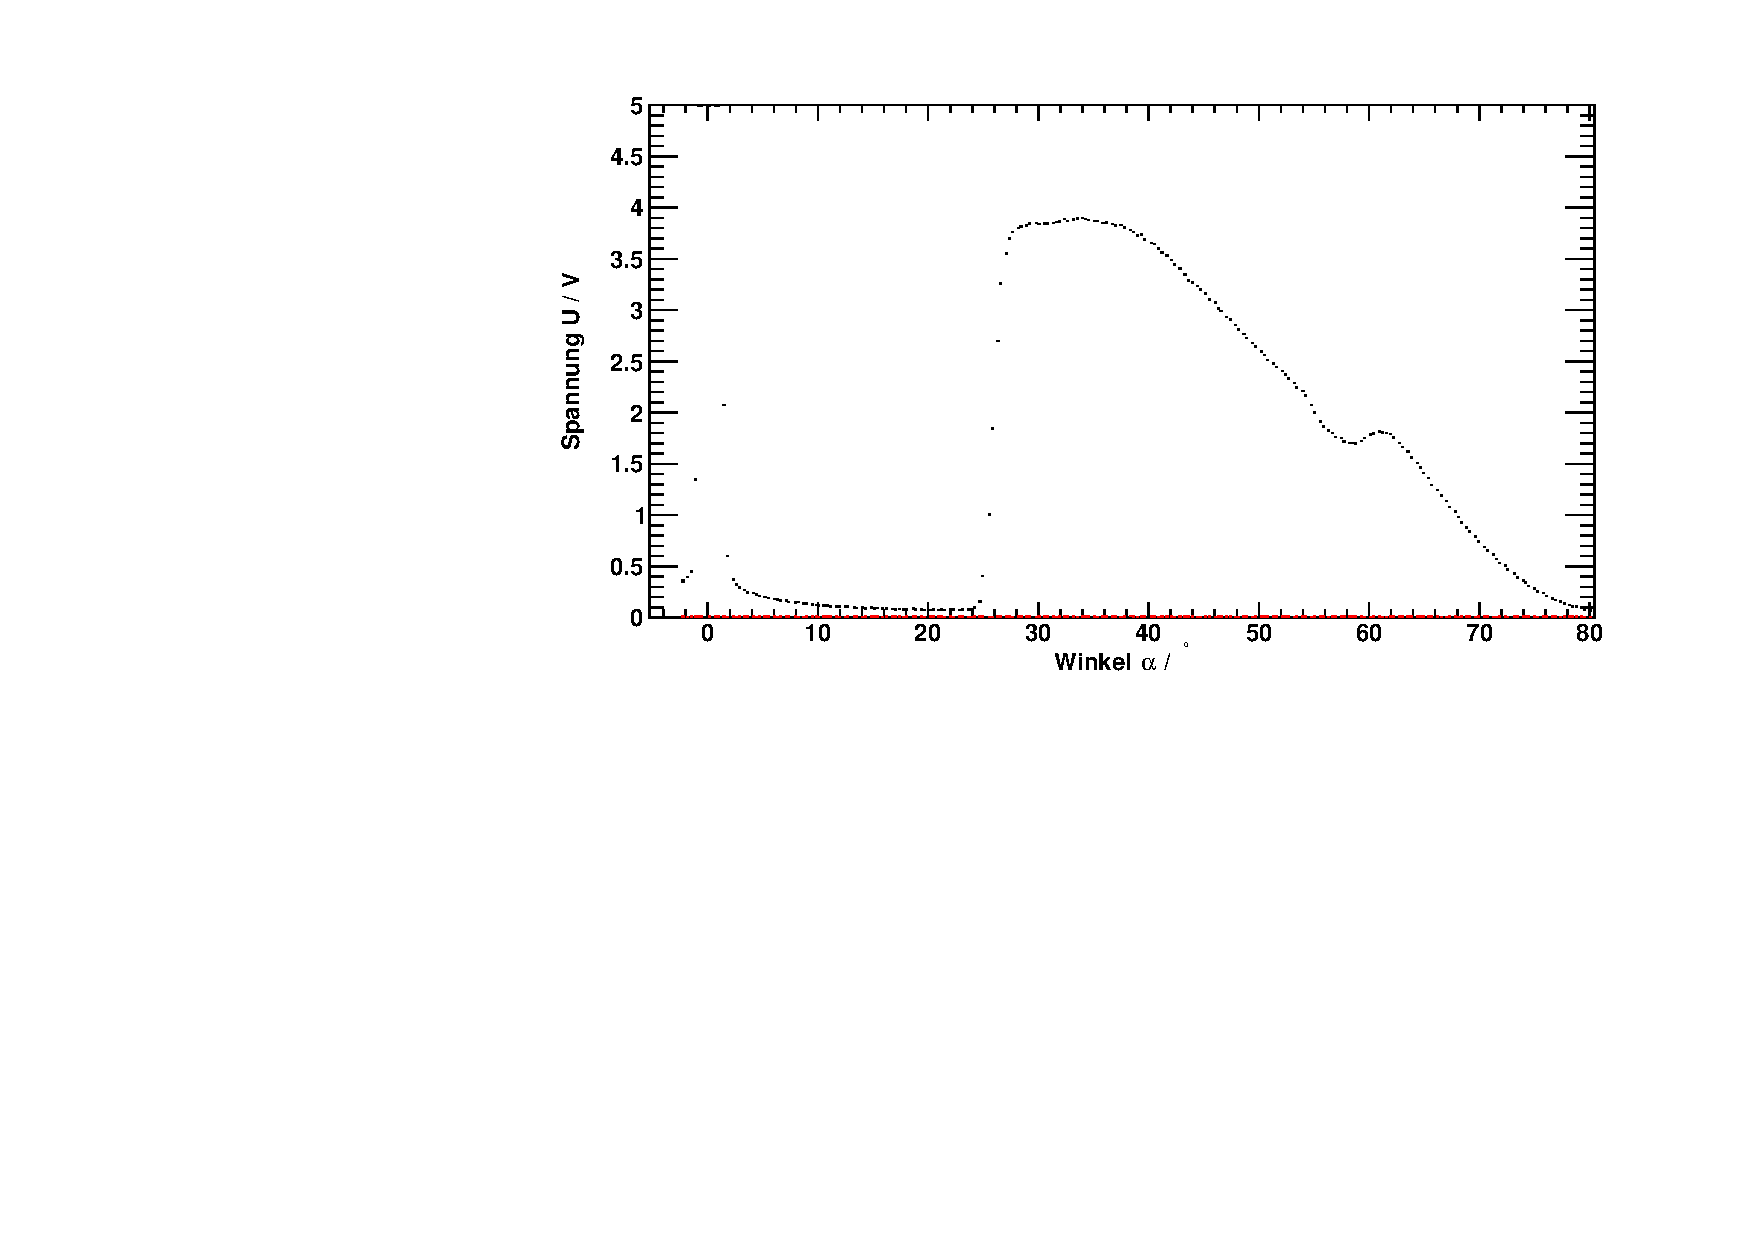
\includegraphics[width=\textwidth]{../img/part1/Si_Lampe_spectrum.pdf}
  \caption{Strahlungsleistung der Lampe in Abhängigkeit des Winkels $alpha$}
  \label{img:si:lampe}
\end{center}
\end{figure}

Die so erhaltenen Intensitäten werden mit den Modellen aus Kapitel \ref{sub:part1:princ:transabs} bei einer Temperatur von $T=300$\,K 
gefittet (\autoref{img:si:transabs}):
\begin{equation}
  \text{Trans}(E) = T_0 \cdot e^{- \alpha(E) \cdot l}, \qquad 
  \text{Abs}(E) = A_0 \cdot e^{- \alpha(E) \cdot d} \left( 1 - e^{- \alpha(E) \cdot (l - d)}  \right) + y_0
\end{equation}

\begin{figure}[H]
\begin{center}
  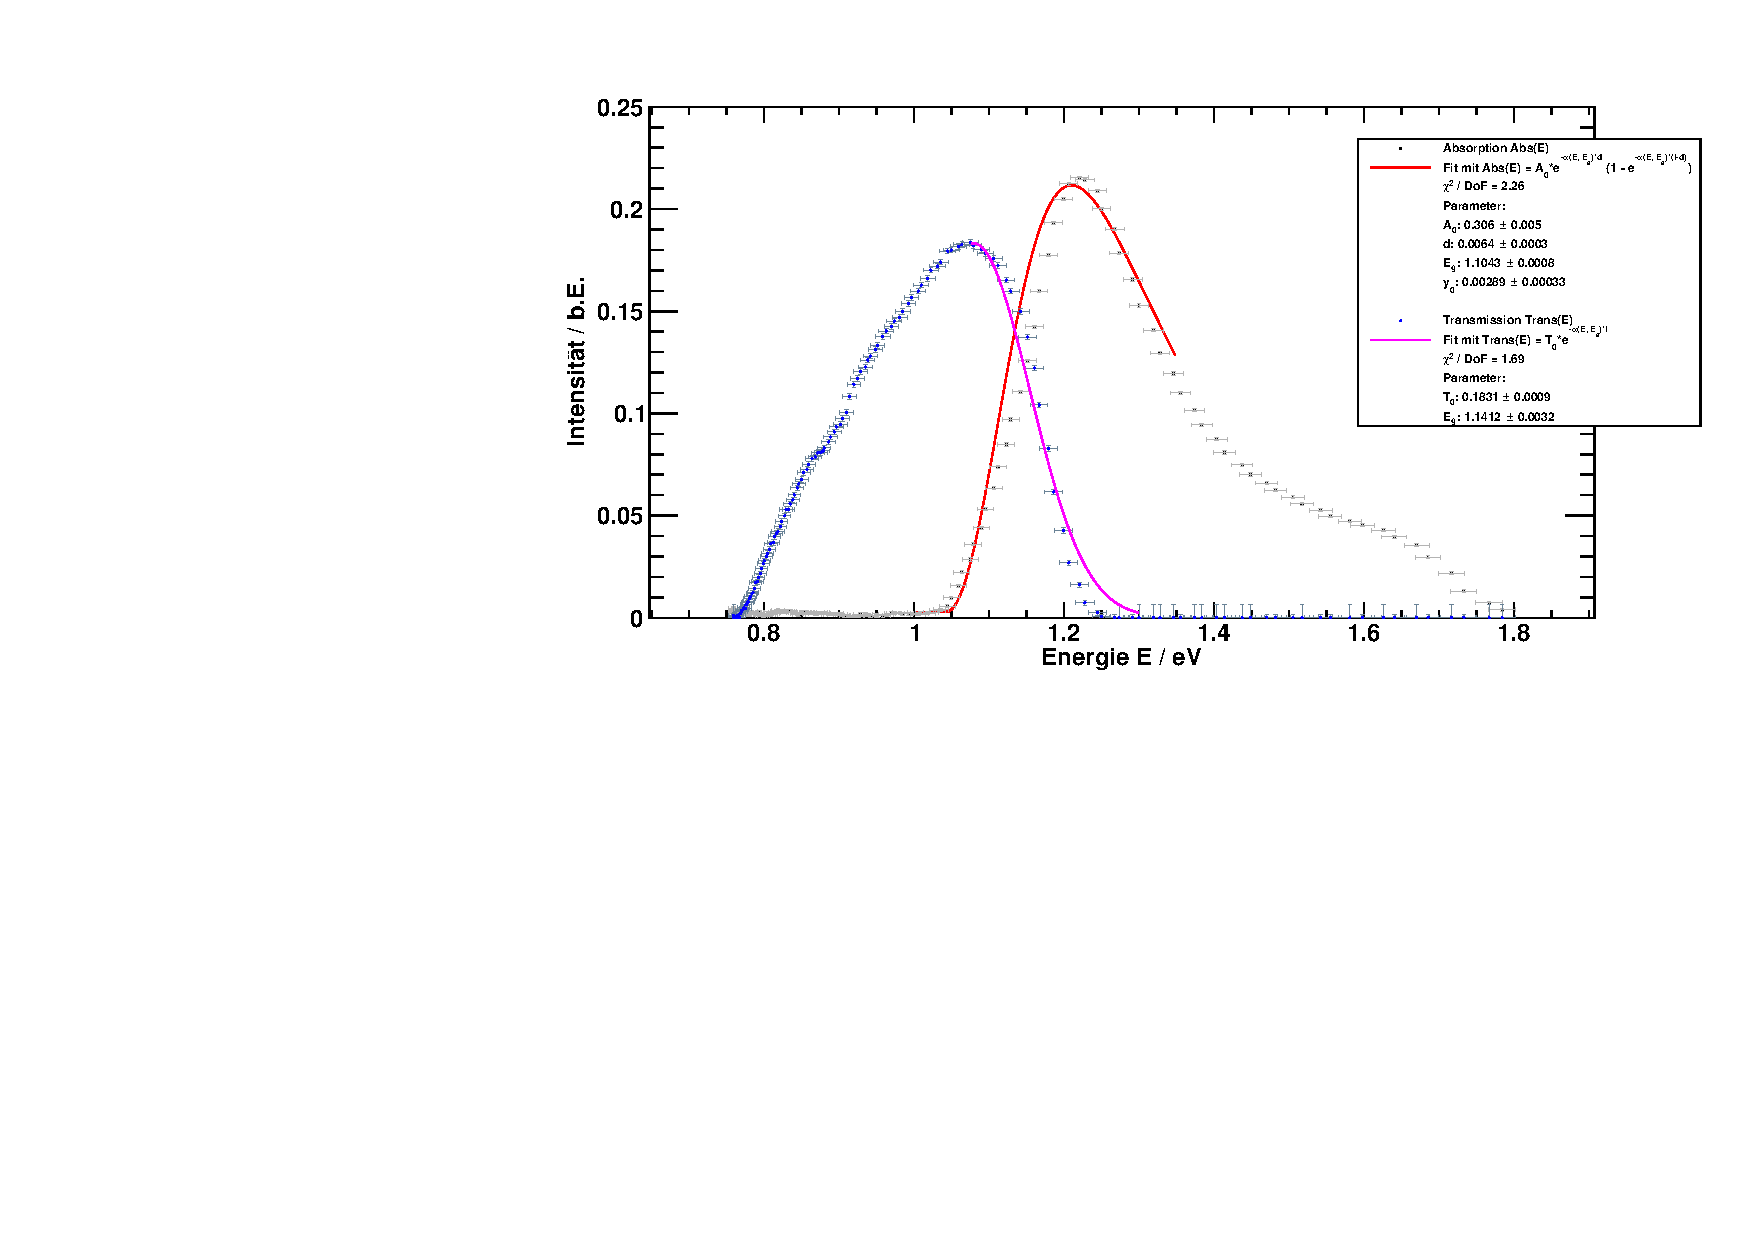
\includegraphics[width=\textwidth]{../img/part1/Si_fit_AbsTrans.pdf}
  \caption{Untergrundbereinigte und normierte Signalintensitäten für die Siliziumprobe.}
  \label{img:si:transabs}
\end{center}
\end{figure}

Man erhält für die Bandlückenenergie von Silizium:
\begin{equation}
\begin{split}
  E_{g, \text{Abs}} &= (1.1043 \pm 0.0008)\,\text{eV} \\
  E_{g, \text{Trans}} &= (1.141 \pm 0.003)\,\text{eV}
\end{split}
\end{equation}
Für den Fehler von $E_g$ muss allerdings noch berücksichtigt werden, dass die endliche Breite der Blende ($d=2$\,cm) und 
des Gitters ($D=2.5$\,cm) nicht eine genaue Energie sondern ein Energieintervall gemessen wird. Nach \cite{staatsex} können 
die Winkel $W_\text{min}$ und $W_\text{max}$ berechnet werden, zwischen denen die Photonen bei einem festen Anstellwinkel $\Phi$ noch 
gemessen werden:
\begin{equation}
\begin{split}
  W_\text{min}(\Phi) &= \Psi + \arcsin \left( \sin(\Psi) - \frac{\frac{D}{2} \cdot \cos(\Phi) + \frac{d}{2} \cdot \cos(\Psi)}{L} \right) \\
  W_\text{max}(\Phi) &= \Psi + \arcsin \left( \sin(\Psi) + \frac{\frac{D}{2} \cdot \cos(\Phi) + \frac{d}{2} \cdot \cos(\Psi)}{L} \right) 
\end{split}
\end{equation}
mit $\Psi=7.5^\circ$ und dem Abstand $L=55$\,cm zwischen Blende und Gitter. \\
Es kann nun der systematische Fehler aus dieser Unschärfe berechnet werden:
\begin{equation}
  s_E = \frac{1}{2} \left( \frac{h \cdot c}{2 \cdot d \cdot \cos(\Psi) \cdot \sin (W_\text{min} / 2)} - \frac{h \cdot c}{2 \cdot d \cdot \cos(\Psi) \cdot \sin (W_\text{max} / 2)} \right) 
\end{equation}
Für den gesamten Fehler auf $E_g$ folgt:
\begin{equation}
  s_{E_g} = \sqrt{s_\text{Fit}^2 + s_E^2}
\end{equation}
Die errechneten Bandlückenenergien können mit \autoref{eq:energy_angle} in den Anstellwinkel $\Phi$ umgerechnet werden. Es folgt für die 
neuen Fehler:
\begin{equation}
\begin{split}
  E_{g, \text{Abs}} &= (1.1043 \pm )\,\text{eV} \\
  E_{g, \text{Trans}} &= (1.141 \pm )\,\text{eV}
\end{split}
\end{equation}
Der gewichtete Mittelwert liefert:
\begin{equation}
  \bar{E}_g = (1.10637 \pm 0.0008)\,\text{eV}
\end{equation}
Die Abweichung vom Literaturwert
\begin{equation}
  E_g^{\text{Lit}} = 1.12\,\text{eV}
\end{equation}
beträgt ca. 1\% des Messwertes. Der Fit liefert nur die statistsichen Fehler 


\subsubsection{Bandlückenenergie von Germanium}
Die Auswertung erfolgt analog zu der Bestimmung der Bandlückenenergie von Silizium. Der Fit (\autoref{img:ge:transabs})
liefert die Bandlückenenergien von Germanium:
\begin{equation}
\begin{split}
  E_{g, \text{Abs}} &= (0.6906 \pm 0.0018)\,\text{eV} \\
  E_{g, \text{Trans}} &= (0.694 \pm 0.002)\,\text{eV}
\end{split}
\end{equation}
%TODO Fehler E_g aus Aufbau
Der gewichtete Mittelwert beträgt
\begin{equation}
  \bar{E}_g = (0.6917 \pm 0.0015)\,\text{eV}
\end{equation}
\begin{equation}
  E_g^{\text{Lit}} = 0.66\,\text{eV}
\end{equation}

\begin{figure}[H]
\begin{center}
  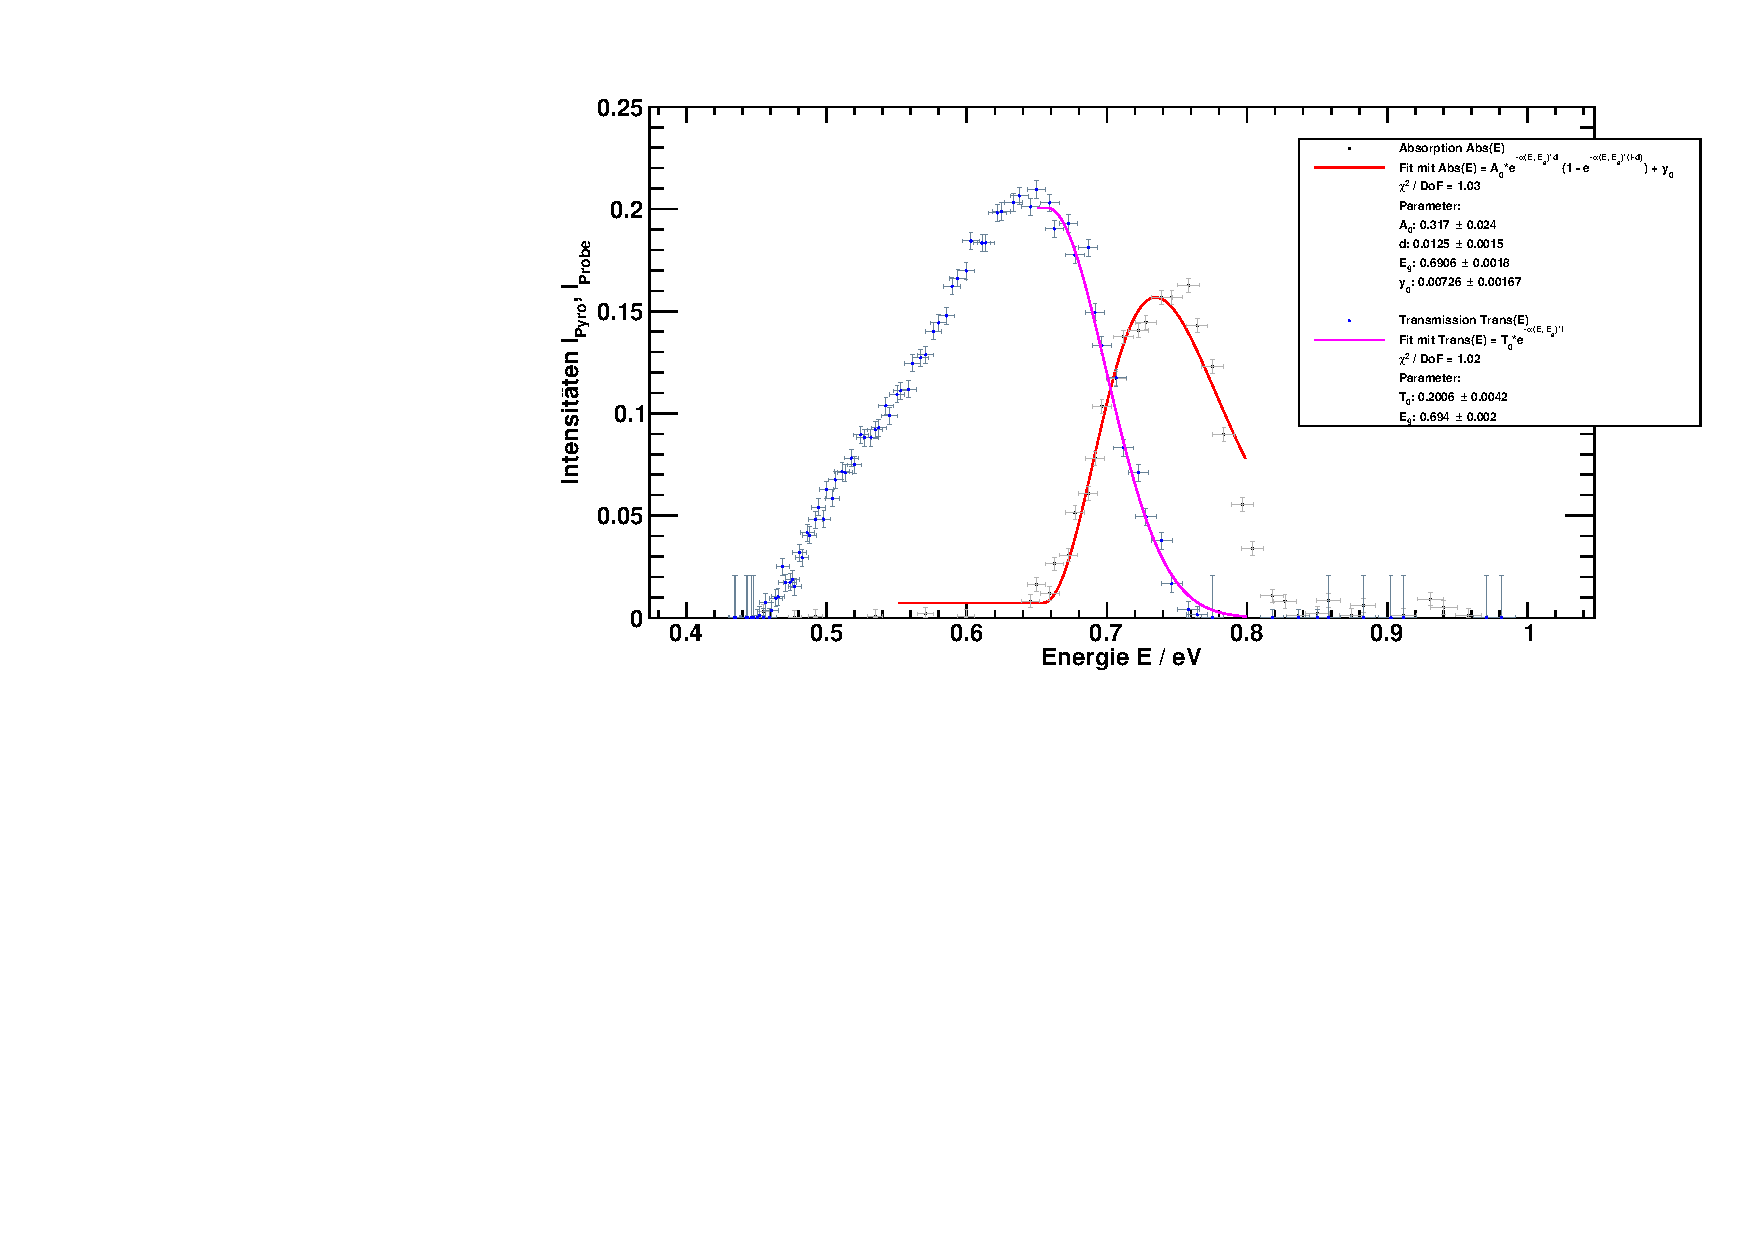
\includegraphics[width=\textwidth]{../img/part1/Ge_fit_AbsTrans.pdf}
  \caption{Untergrundbereinigte und normierte Signalintensitäten für die Germaniumprobe.}
  \label{img:ge:transabs}
\end{center}
\end{figure}
